\documentclass{sig-alternate-10pt}

\usepackage{times}
\usepackage{graphics}
\usepackage{listings}
\usepackage{subfigure}
\usepackage{booktabs}
\usepackage{colortbl}
\usepackage{tabularx}
\usepackage{color}
\usepackage{xspace}
\usepackage{hyperref}    % Creates hyperlinks from ref/cite
\hypersetup{pdfstartview=FitH}
\usepackage{graphicx}    % For importing graphics
\usepackage{url}         %
\usepackage{caption}

\hypersetup{%
pdftitle={Latency Measurement and Analysis of Wide Area, Data Center, and Mobile Networks}, pdfauthor={Ben Zhang, Ahir Reddy}, pdfkeywords={Internet, Latency, Measurement}, bookmarksnumbered, pdfstartview={FitH}, colorlinks,
citecolor=black, filecolor=black, linkcolor=black, urlcolor=black,
breaklinks=true,}

\renewcommand{\arraystretch}{1.2} % Space out rows in tables

\newcommand{\ml}[1]{{\color{green} {\it ML: #1}}}

% No space between bibliography items:
\let\oldthebibliography=\thebibliography
  \let\endoldthebibliography=\endthebibliography
  \renewenvironment{thebibliography}[1]{%
    \begin{oldthebibliography}{#1}%
      \setlength{\parskip}{0ex}%
      \setlength{\itemsep}{0ex}%
  }%
  {%
    \end{oldthebibliography}%
  }

%\pagenumbering{arabic}  % Arabic page numbers for submission.  Remove this line to eliminate page numbers for the camera ready copy

\begin{document}

% use this command to override the default ACM copyright statement
% (e.g. for preprints). Remove for camera ready copy.
%\toappear{Submitted for review to IPSN 2012.}
% \conferenceinfo{ConfName} {Date, Location}
% \CopyrightYear{Year} 
% \crdata{978-1-4503-1227-1/12/04} 
% \clubpenalty=10000 
% \widowpenalty = 10000


% to make various LaTeX processors do the right thing with page size
\special{papersize=8.5in,11in}
\setlength{\paperheight}{11in}
\setlength{\paperwidth}{8.5in}
\setlength{\pdfpageheight}{\paperheight}
\setlength{\pdfpagewidth}{\paperwidth}

\setlength{\textfloatsep}{13pt plus 2pt minus 1pt}

\title{Latency Measurement and Analysis of Wide Area, Data Center, and Mobile Networks}

\author{
{Ben Zhang, Ahir Reddy}\\
\affaddr{University of California, Berkeley}\\
%\affaddr{}\\
\email{benzh@eecs.berkeley.edu, ahirreddy@berkeley.edu}
}

\maketitle

\begin{abstract}
% Abstract for measurement project.
Understanding the current state of Internet performance is critical to both academic research and industrial systems. Though various metrics (connectivity, available bandwidth, etc.) are important to evaluate, in this project, we focus on the latency of current Internet (as of 2013) in the Wide Area Network (WAN), Data Center, and Cellular Networks.

We employed the King/Turbo-King methods proposed in the literature to measure the latency between two arbitrary hosts. The correlation of latency with geographical location will allow for identification of the gap between existing network performance and the speed-of-light limit. Such data serves as the starting point for analyzing wide area network performance. As the number of services deployed in the cloud continues to increase, latencies experienced by end-users are increasingly dependent on data center performance. We use Google Search in our case study to understand the composition of time in typical data center queries. The our final study explored cellular networks; more specifically we evaluated AT\&T's 4G-LTE network in the Bay Area. We utilized {\it traceroute} to test the latency of the new flat IP architecture in LTE networks.

\end{abstract}

%\category{C.2.1}{Computer-Communication Networks}{Network Architecture and Design}[Wireless communication]
%\keywords{Collection, CTP, Sensor Network, Routing}

% \category{B.0}{Hardware}{General}
% \category{B.4}{Hardware}{Input/Output \& Data Communication} 
% \category{H.4.m}{Information Systems Applications}{Miscellaneous}

% \terms{Design, Experimentation, Measurement} 
\keywords{Internet Latency, Measurement Study, King, Turbo King, Planet Lab, traceroute}

\section{Introduction}
\label{sec:introduction}

The measurement of Internet has become increasingly important and challenging due to its complexity, large-scale and variability. A numbers of tools have been proposed to accomplish this task (see Sec.\,\ref{sec:related-work} for a complete review). In this project, our primary goal is not to introduce any novel network measurement tool; instead, we use existing measurement techniques to characterize the performance of current Internet. We base our work on previous investigations, and try to elucidate the changes in measurement strategies and outcomes. Specifically, the cloud computing service model and mobile computing have re-shaped the Internet in unanticipated ways. The impact of these new models on end-to-end latency and measurement techniques have never been formally studied. We propose the questions listed bellow as motivations for our study.

\begin{itemize}
\item How does network latency vary among different kinds of end hosts -- generic end users(including mobile/wireless end hosts), regular web servers, and cloud service from data centers?
\item How current Internet latency performs in comparison to the speed-of-light limit?
\item How wide-area networks and data centers contribute to end-to-end latency experienced by end users?
\item How the latency is affected by edge caching of content, especially on mobile networks?
\item What are the characteristics of time-series analysis for latency on a daily/weekly/yearly basis?
\end{itemize}

Our initial approach will consist of re-implementing and re-producing previous measurement works in the context of current Internet, following the guidelines outlined in \cite{paxson2004strategies}. One major strategy we intend to re-implement is King \cite{gummadi2002king}, a strategy which leverages the DNS infrastructure to measure end-to-end latency of arbitrary end hosts. To guarantee deliverables, we have a outlined an initial timetable for our study below(see Table.\,\ref{tab:plan}).

\begin{table}
  \centering
  \begin{tabular}{ c|p{4cm} }
    \hline
    Period & Task \\
    \hline
    Late Feburary & Literature review \\
    March & Re-implementation and initial measurements \\
    April & Revision/correction of any possible methodology flaws \\
    Early May & Wrap up and report \\ 
    \hline
  \end{tabular}
  \label{tab:plan}
  \caption{timeline for project}
\end{table}

%%% Local Variables: 
%%% mode: latex
%%% TeX-master: "main"
%%% End: 

\section{Related Work}
\label{sec:related-work}

Describe related work here.

%
\section{Expected Results}
\label{sec:results}

We expect to have results in the form of actual measurement tools and data, as well as analysis tools and reproducible analysis output. The dataset will consist of latency measurements between end hosts along with meta-data (the DNS query, Geo-IP resolution, time of testing, environment of testing, etc.). Our analysis will compare latency to time and physical location, and separate WAN latency from datacenter latency.

%%% Local Variables: 
%%% mode: latex
%%% TeX-master: "main"
%%% End: 

\section{Latency in WAN}
\label{sec:latency-wan}

\subsection{Methodology}
\label{sec:methodology}


We derive our measurement methodology from King \cite{gummadi2002king} and Turbo-King \cite{leonard2008turbo}, and developed a Turbo-King variant illustrated in Fig.\,\ref{fig:king_model}. The King method leverages DNS name-servers to make measurements that approximate latency between arbitrary end hosts. It utilizes properties of DNS to coerce recursive DNS resolvers into making outbound queries on behalf of measuring party. Turbo-King builds upon King by allowing for detection of DNS forwarders. DNS forwarders aggregate DNS queries within a network that target external DNS servers and can serve responses. The original King method has no means of detecting these servers, and as a result they may skew measurement results.

\subsubsection{Overview}
Our methodology is composed of 4 elements, a measurement node, a central domain name server, and 2 target name servers. A measurement nodes is composed of a DNS client and server. A node accepts remote-procedure calls that specify 2 target DNS servers and returns both DNS latency measurements and multiple round trip time calculations to the first target server. The central domain name server simply refers incoming DNS requests to the originating measurement node. The 2 target name servers must have known locations and the first must be an open-recursive resolver. Below we outline the measurement process.

\begin{enumerate}
	\item DNS Client on measurement node will issue a request to the first target DNS server. The requested URL will be of the form "qid.myAddr.mydomain.com", where qid is the query id, myAddr is an encoding of the measurement nodes public name, and mydomain is the domain controlled our central name server.
	\item The target server will issue a request containing the requested URL to the central name server
	\item The central name server will decode the "myAddr" element of the requested URL to the url of the originating measurement node. It will return a response to the querying target server with a referral to the measurement node.
	\item The target name server will then issue a DNS query with the requested URL to the measurement node.
	\item The measurement node will receive a DNS query, lookup the query id and return a referral with the corresponding second target DNS server.
	\item The first target DNS server will issue a request to the second DNS server
	\item The second server will deliver a response (to be discussed more)
	\item The first target name server will then pass along this response to the DNS client of the measurement node.
\end{enumerate}

We record the time delta between step 5 and 8, and subtract the round-trip time between the measurement node and the first target to generate a latency measurement between the two target DNS servers.

\subsubsection{Round Trip Time Latency}
To determine the round trip latency between a measurement node and the first target server, we issue a DNS query for a random subdomain in the domain controlled by the target name server. We issue this request multiple times to allow and discard the first measurement. In this way we allow for the request to be cached on the target server and minimize the processing time to generate more accurate round-trip time measurements. We adopted This method is over ICMP ping because a fraction of DNS servers we queried did not respond to ICMP requests.

\subsubsection{Additional Considerations}
It is important to note that upon the first DNS request to the second target DNS server, that server itself may try a complete resolution if it is an open resolver. In this case, the second target server will issue a request to resolve our domain and will be referred to the originating measurement node. It will issue a request to this node that contains the original query id; in this event the measurement node will not issue a response and allow the second target server to time out. The second target will then return a NXDomain response to the first target name server, and upon subsequent requests for our domain (within some time period dictated by that servers caching policy) it will issue continue to issue error responses. Thus, we always discard the first latency measurement in every round to account for this additional lookup latency.

\begin{figure}
  \centering
  \includegraphics[width=\linewidth]{../figs/king_model.pdf}
  \caption{King/T-King method illustration}
  \label{fig:king_model}
\end{figure}

\subsubsection{Reverse DNS Crawl}
The Turbo-King methodology requires a large set of known open recursive name servers to generate latency measurements. An open recursive name server will respond to requests for any arbitrary domain from clients outside its AS. Only the first target name server must be an open resolver, the second server may be any DNS server that issues any response to external queries. To build a set of DNS servers, we performed a crawl of the reverse DNS tree.

Reverse DNS requests take the form of requests for the ".in-addr.arpa" prefixed in reverse order with the octets of the IP to be resolved. Queries operate as normal DNS queries do, where in each octet is a sub-domain for which a DNS server is responsible for.
At the first level of the DNS tree we issue a query to the "in-addr.arpa" domain for the first octet (1-255) and receive responses (start of authority, SOA, records) that indicate the servers responsible for the next level of the tree. We continue by issuing requests for the second octet (second.first.in-addr.arpa) to these servers, and we proceed similarly for the third octet. If we do not receive an SOA record skip further search down the tree that contains that prefix. At each step, we record any responses that indicate authoritative name servers. Thus, after a three level traversal we are left with a set of authoritative DNS servers. We implemented and deployed a multi-threaded crawler to Amazon EC2 that was able to complete a traversal on the order of 1 day.

\subsubsection{Open Resolvers}
Our methodology requires that the first DNS resolver be an open recursive resolver. To build this set, we leverage the service provided by the DNS Measurement Factory. By issuing a DNS query to the Measurement Factory name server it will check if that server is an open resolver and return the results.\cite{dnsfactory}

\begin{figure}
  \centering
  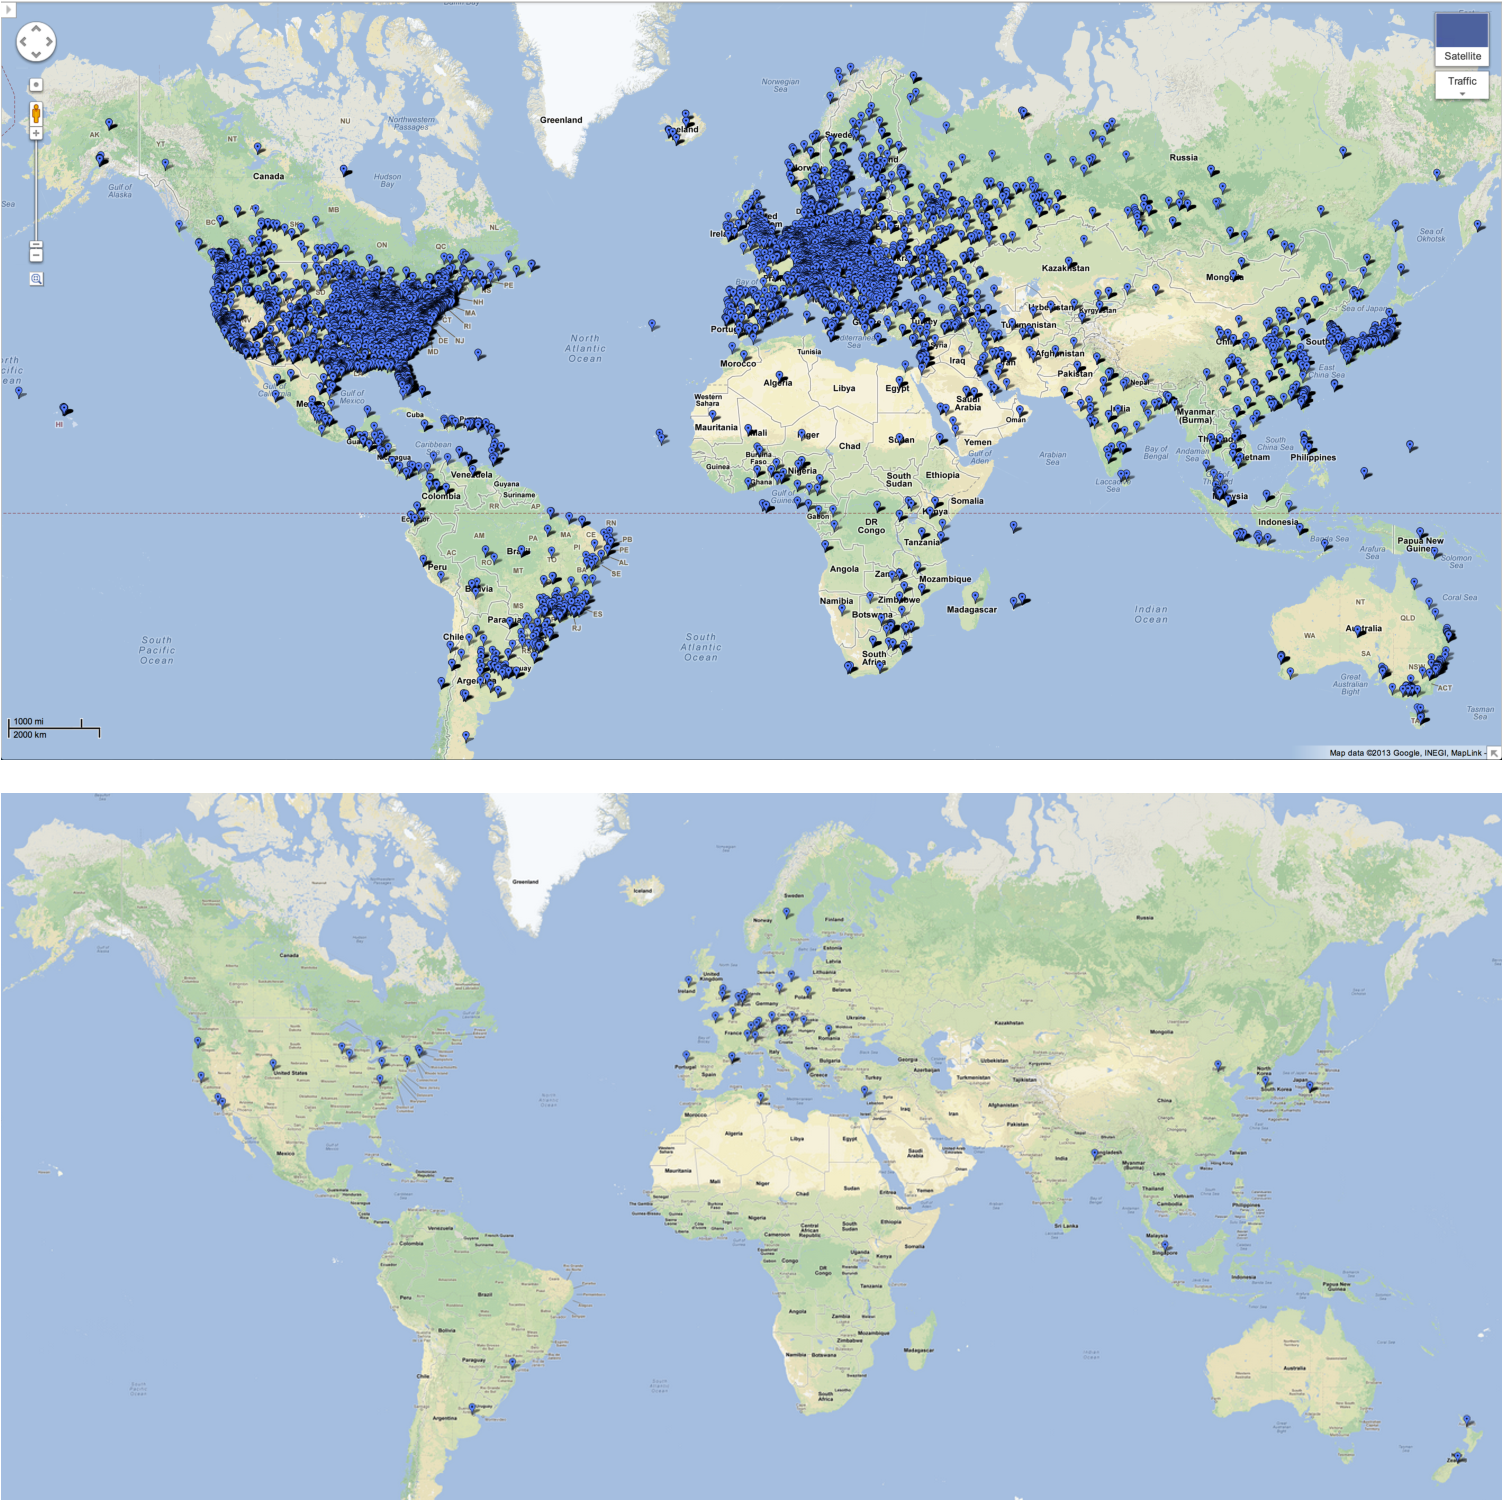
\includegraphics[width=\linewidth]{../figs/geo_viz.pdf}
  \caption{(Top) Distribution of open resolvers, visualized using Google Map, (Bottom) Distribution of PlanetLab nodes that we are using, visualized using Google Map}
  \label{fig:geo_viz}
\end{figure}


\subsection{Implementation and Experiment}
\label{sec:impl-exper}

Using a combination of EC2 and Planet Lab servers, we collected approximately x.xx successful measurement results between 4/20/13 and 5/4/13.

\subsubsection{Measurement Node}
We utilized the dnspython libraries to implement our Turbo-King variant. Each measurement node runs a Turbo-King server (composed of a DNS client and server) which exposes a remote procedure call service using the RPYC library. We deployed the Turbo-King server to 56 Planet Lab nodes (Fig. X).

\subsubsection{Central Name Server}
Our central name server is implemented using the Python twisted framework, which allowed for highly parallel and asynchronous handling of DNS queries. We deployed 2 name-servers on Amazon EC2.

\subsubsection{Controller}
Latency measurements were centrally managed from a controller running on EC2. The controller is responsible for issuing remote-procedure calls to Turbo-King servers and storing the resulting data. The controller randomly selects 2 target name servers, the first from the set of open recursive resolvers, and the second from the set of all resolvers. It then determines the 10 nearest Turbo-King servers to the first target, issues a remote procedure call to each, and stores the results in a relational database. The controller is composed of multiple threads that follow this procedure and run continuously.

\subsection{Analysis}
\label{sec:analysis}

\subsubsection{Distribution of Distances}
Figure \,\ref{fig:latency_distance_distribution} represents the distribution of distances between target DNS servers in the collected measurements. It is interesting to note that the distribution is bimodal (peaking at 1000km and 8000km). We believe this property is reflective of the inter and intra continental patterns in our DNS resolver set (fig.\,\ref{fig:geo_viz}). Resolvers are concentrated in USA and Europe, and as such we believe the high probability of randomly selecting a USA to USA or Europe to Europe target pair generates the first peak of the measurement distribution. Similarly, the second peak is generated by a USA to Europe (or vice versa) target pair.

\subsubsection{Latency vs. Distance}

\begin{figure*}
  \centering
  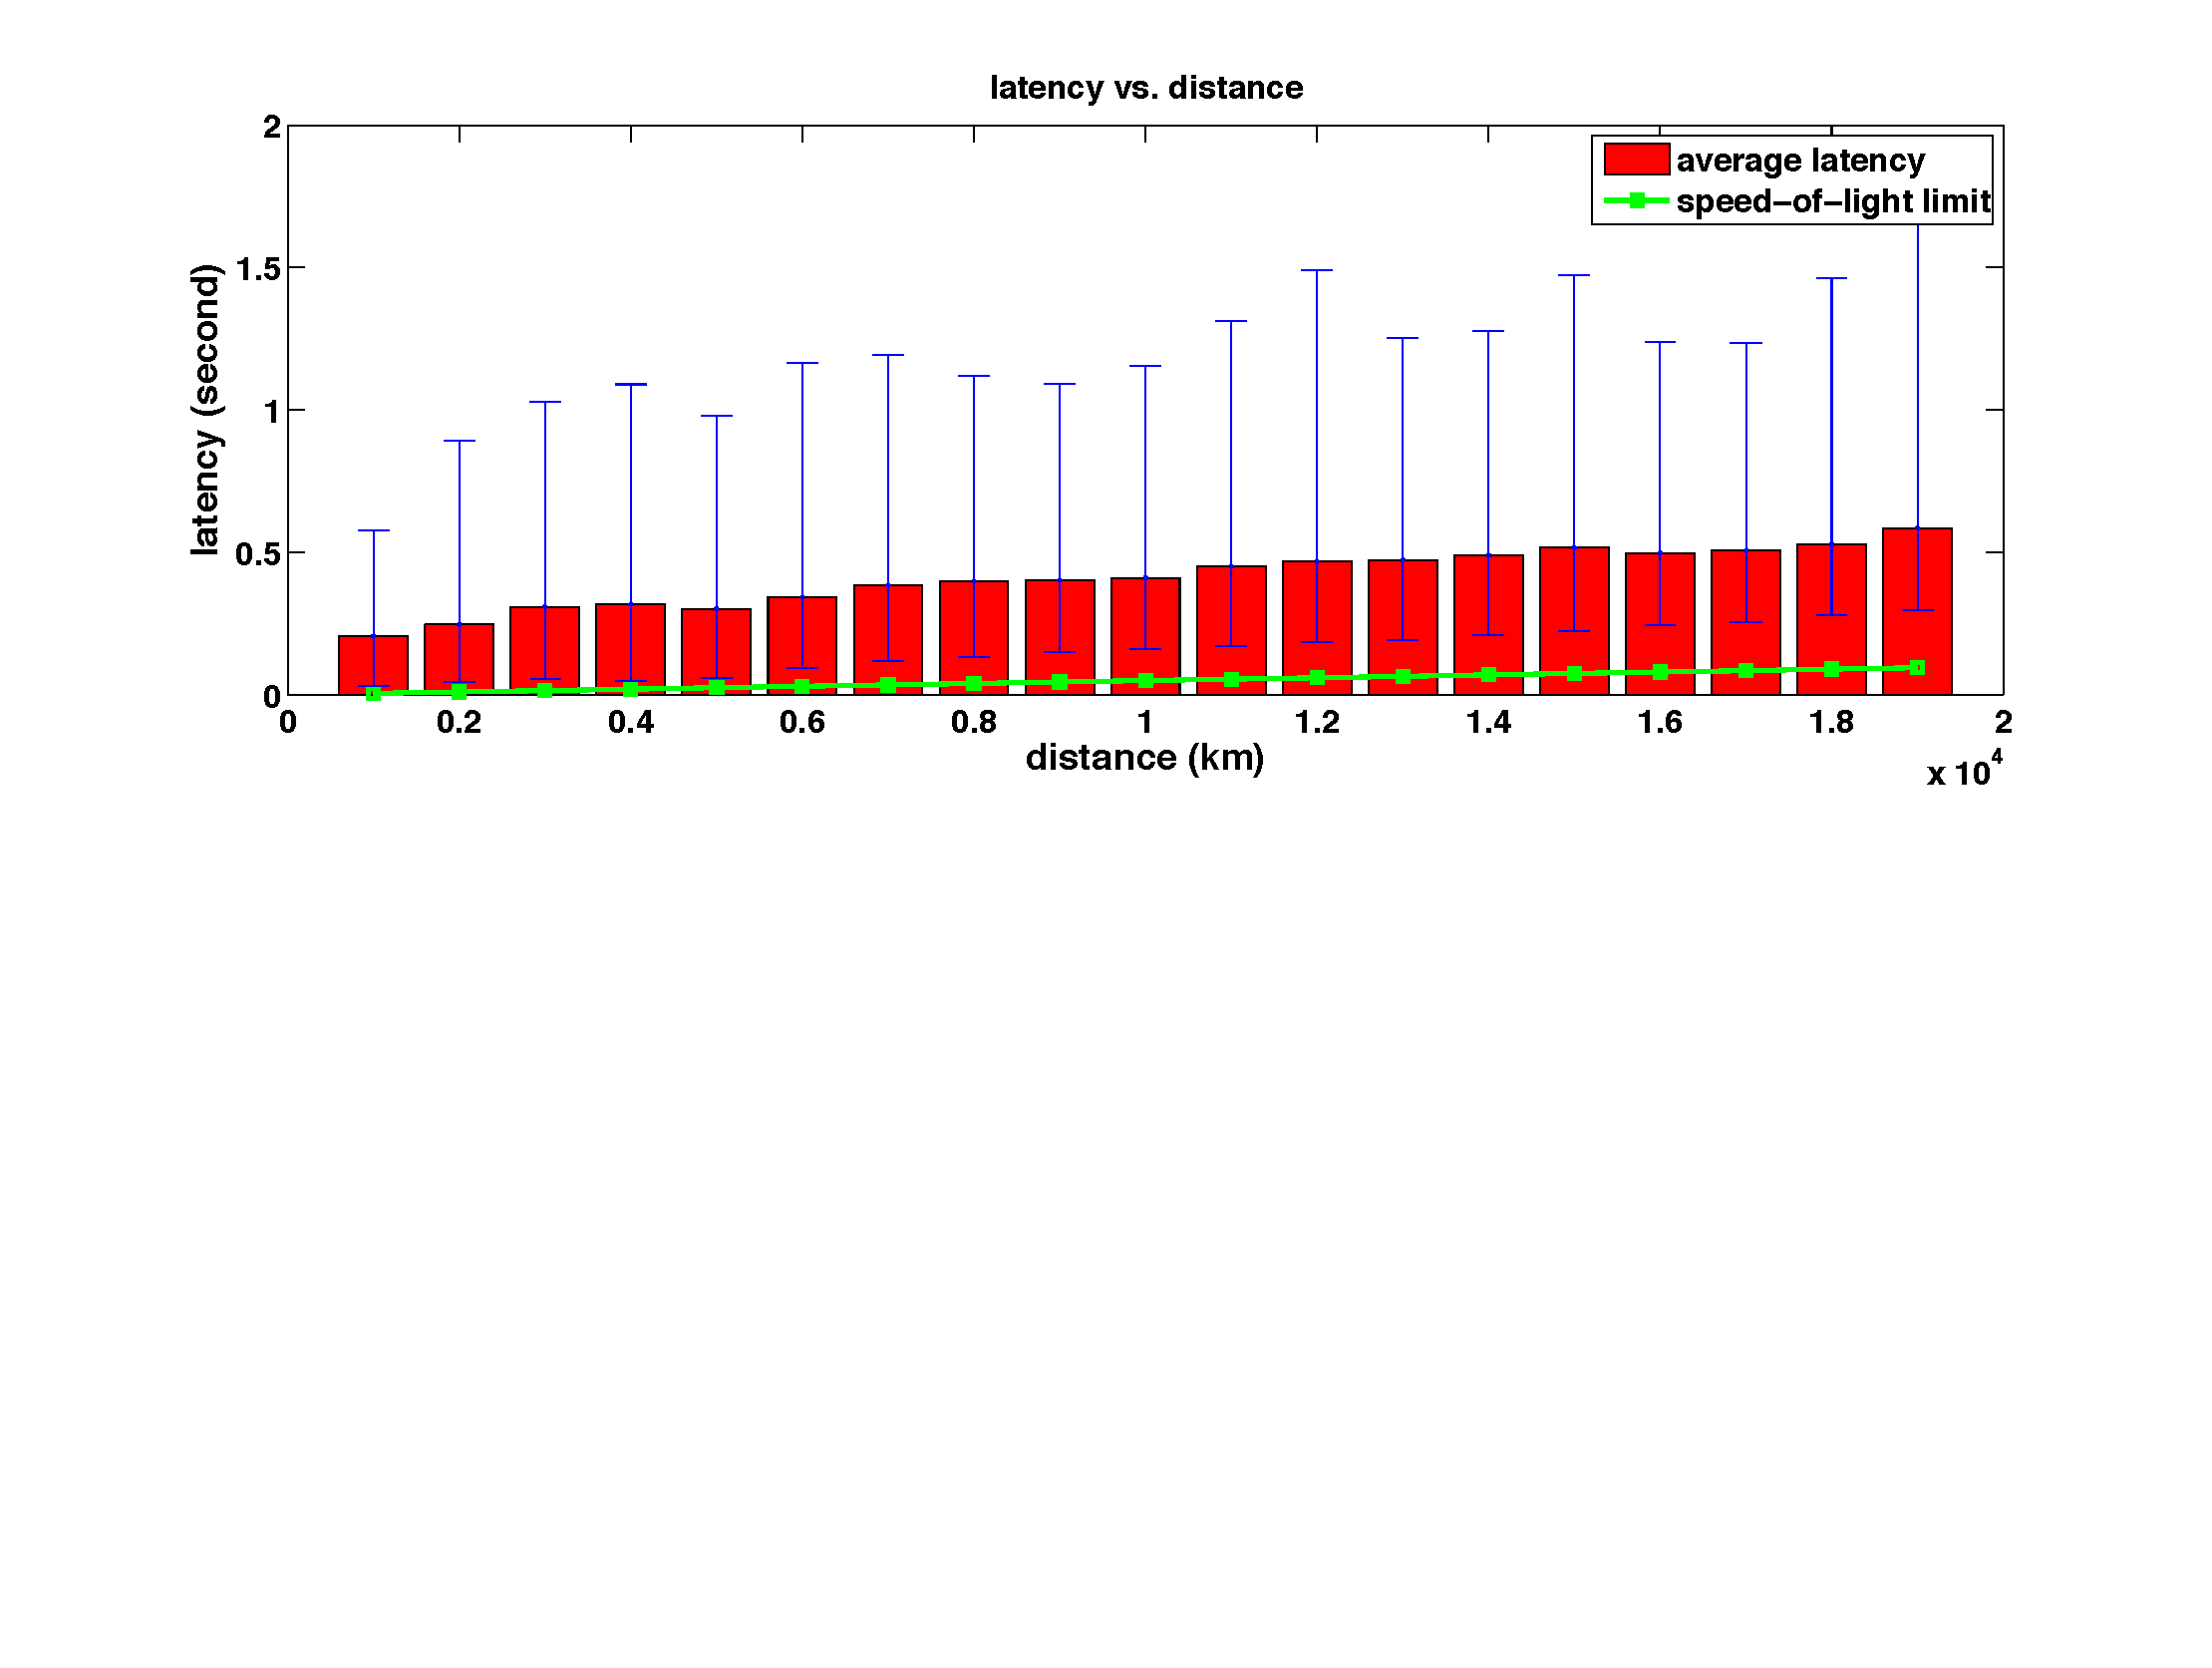
\includegraphics[width=\linewidth]{../figs/King_latency_dist.pdf}
  \caption{Latency vs. Distance}
  \label{fig:latency_dist}
\end{figure*}

\begin{figure}
  \centering
  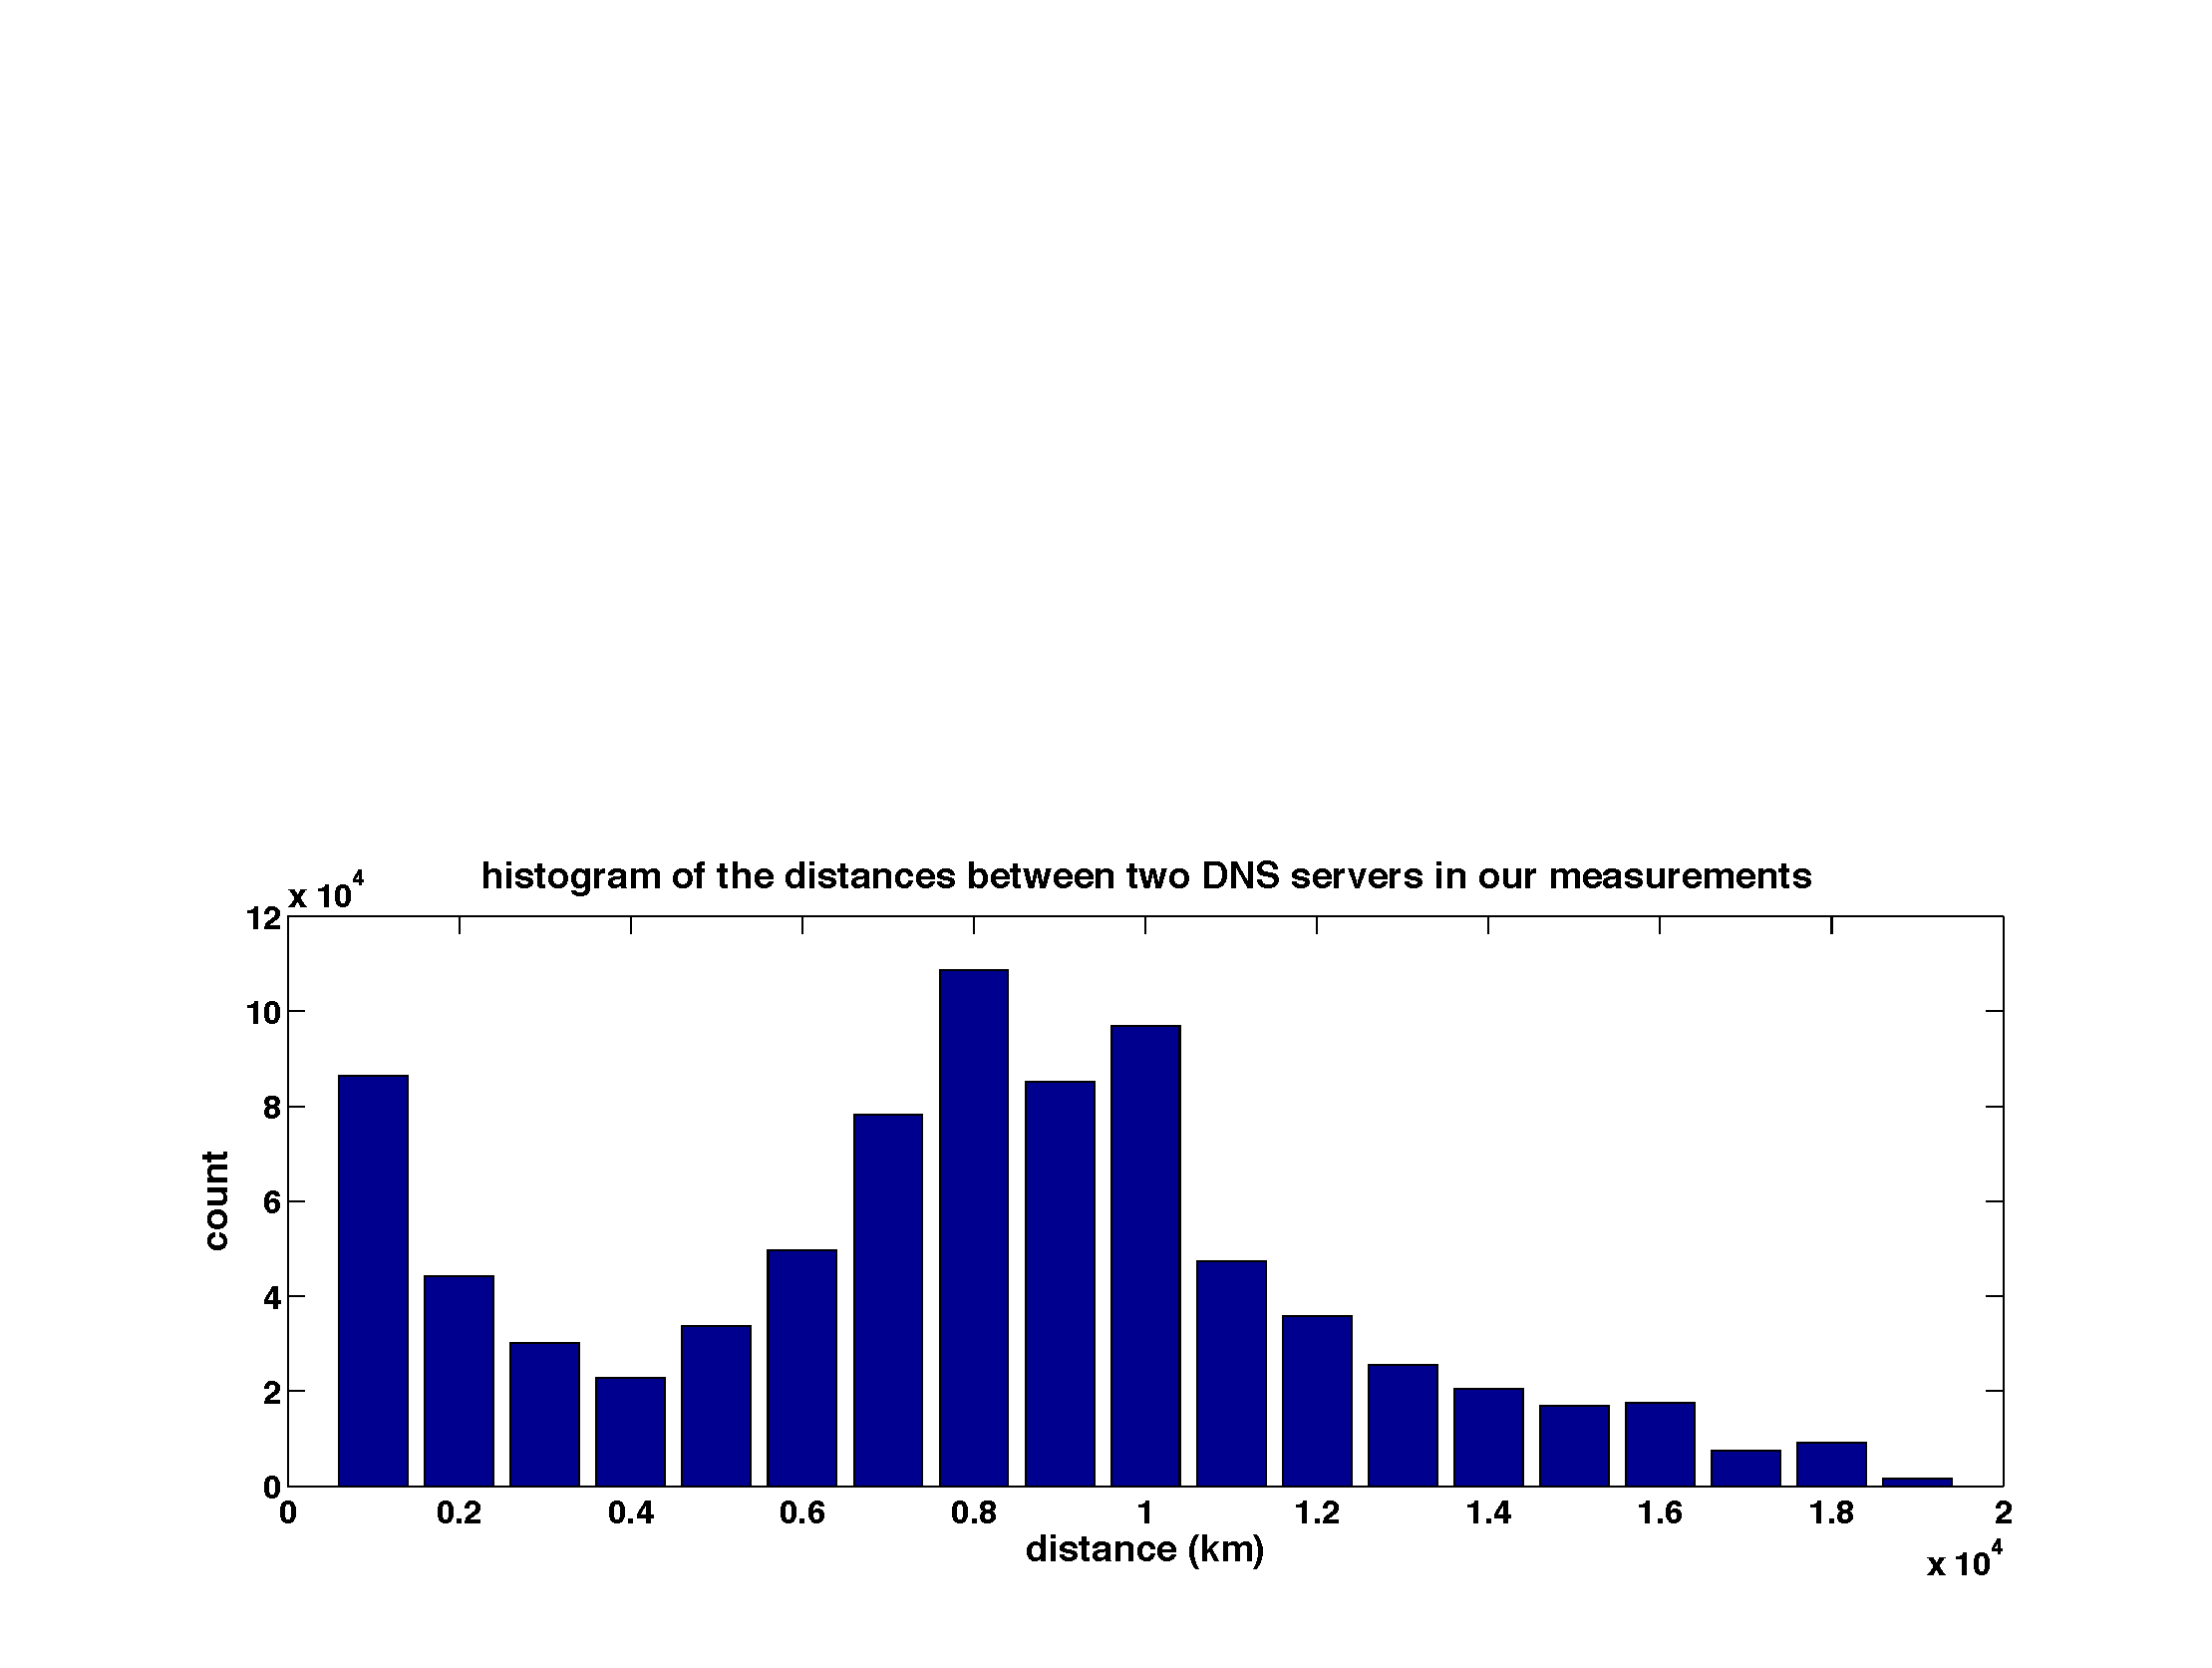
\includegraphics[width=\linewidth]{../figs/King_distance_distrbution.pdf}
  \caption{Distribution of distances of measured latencies}
  \label{fig:latency_distance_distribution}
\end{figure}

\begin{figure}
  \centering
  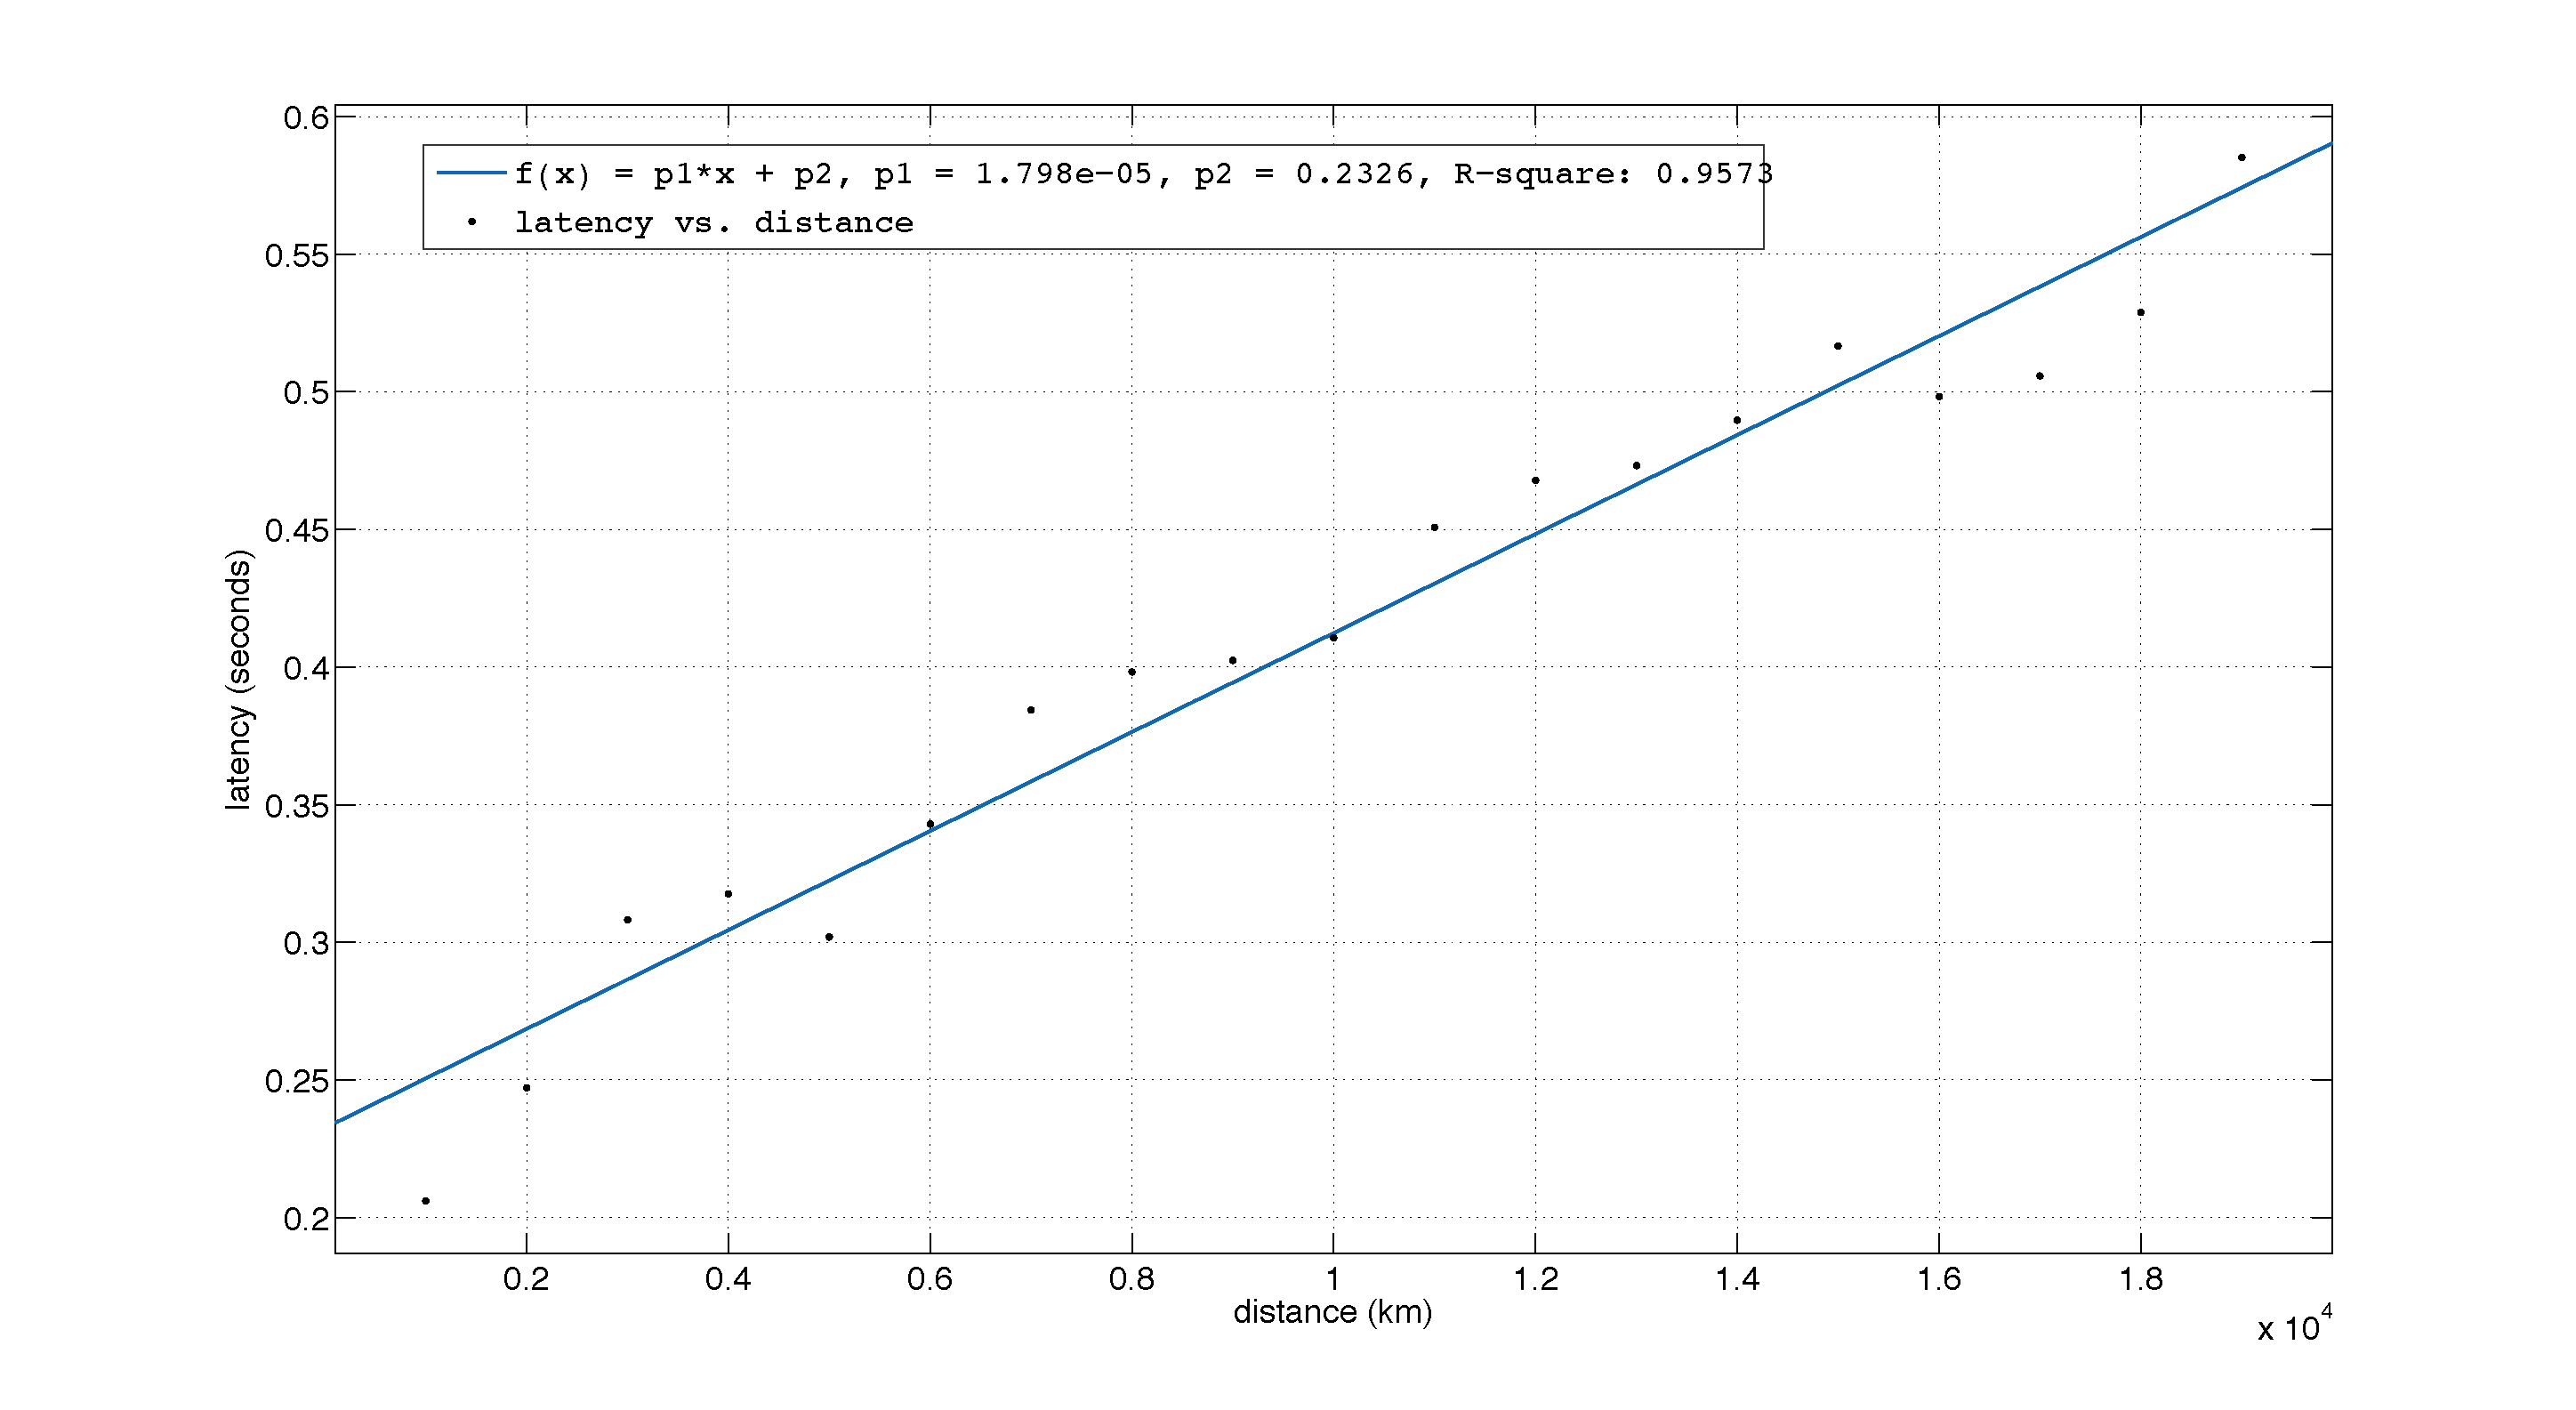
\includegraphics[width=\linewidth]{../figs/fit_curve.pdf}
  \caption{Linear fitting of latency vs. distance}
  \label{fig:fit_curve}
\end{figure}


%%% Local Variables: 
%%% mode: latex
%%% TeX-master: "main"
%%% End: 

\section{Latency for DC conversations}

\subsection{Methodology}

Bearing in mind that the primary goal for this part is to understand the partition of latency from end-users' perspective, we designed the experiment to perform data center related tasks. We expect the model in Fig.\,\ref{fig:DC_model} to be used, and the fractions in the WAN and the DC are also shown. 

\begin{figure}
  \centering
  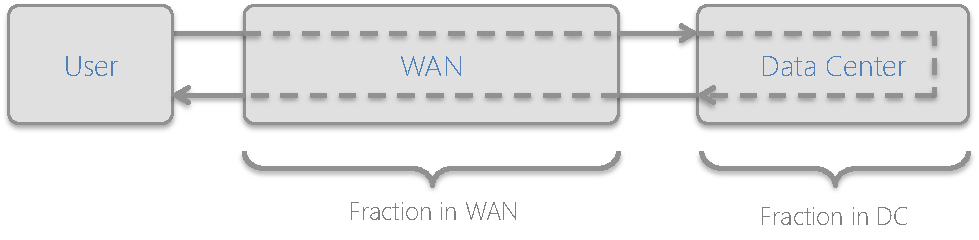
\includegraphics[width=\linewidth]{../figs/DC_model.pdf}
  \caption{Typical user-DC communication pattern}
  \label{fig:DC_model}
\end{figure}

As an representative user-facing service, we have chosen Google Search as the case study. One of the reason of choosing Google Search is that they provide an estimated time spent within their DC (Fig.\,\ref{fig:google_time}). From our analysis in Sec.\,\ref{sec:analysis}, this data is fairly accurate in reflecting the fraction in DC. 

\begin{figure}[t]
  \centering
  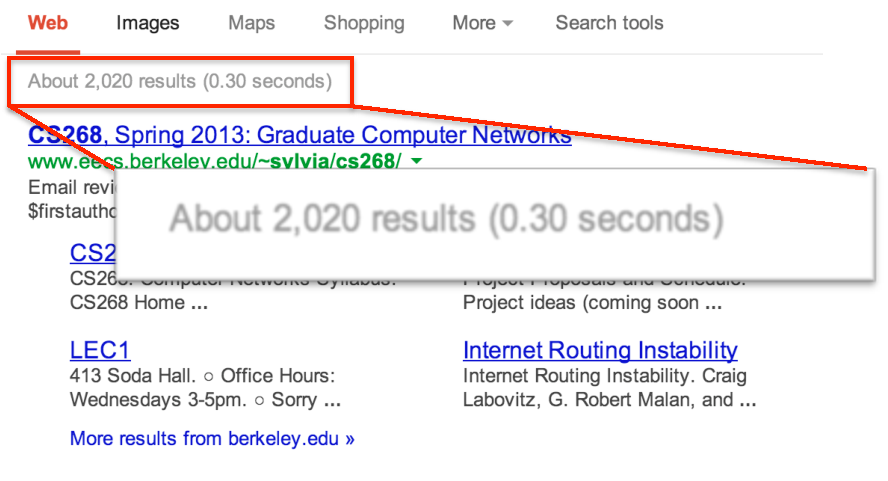
\includegraphics[width=0.85\linewidth]{../figs/GoogleTime.pdf}
  \caption{Google Search estimated time spent within Google in the return webpage}
  \label{fig:google_time}
\end{figure}

To measure the time for a single query, this can be easily done at the end-host side by timestamping the start and end of each query. But what to query remains a problem. Initially, we were suspecting that caching might happens at the Internet-facing router in DC. Querying the hottest words which are likely to be cached might reveal the WAN fraction. On the other side, to force the query to be processed by the DC (eliminating caching), we use random string for search. The hottest words can be found in Google Trends\footnote{http://www.google.com/trends/hottrends}, and we generate random strings comprised of lower cases, upper cases and numbers with length 32. Though the analysis in Sec.\,\ref{sec:analysis} shows a different results instead of what we have expected. This methodology is still useful to understand the problem we are initially planning to solve. 

In the meantime, {\it ping} is performed to measure the networking latency from the user to Google. Since we plan to conduct this experiment in geographically distributed fashion, and Google has many user-facing servers/IPs, we have to make sure we are measuring the right one. In this case, in additional to application layer HTTP conversation, we use {\it tcpdump} to capture all the packets and find out Google's IP address to ping.
 
In summary, to conduct the WAN vs. DC measurement, we issue query to Google and measure four different ``times'', shown in Table.\,\ref{tab:DC_method}.

\begin{table}
  \begin{tabular}{p{2.8cm} | p{5cm}}
    \hline
    type & description \\
    \hline
    Hot-trend-query time & the time spent to query a hot trend word to Google. \\
    Random-query time & the time spent to query a 32-character random string.  \\
    Ping time & the networking layer round-trip time to the responded Google IP address. \\
    Google time & Google's estimated time spent within their DC. \\
    \hline
  \end{tabular}
  \caption{Four different ``times'' measured}
  \label{tab:DC_method}
\end{table}

\subsection{Implementation and Experiement}
\label{sec:impl-exper}

We implement this measurement script in Python, and use {\it cron} to schedule the execution every two hours. Each time, the script will first visit Google Trends webpage and obtain the hot-trend words for that hour. Together with random generated strings, we obtain a list of 20 words for query. The entire list is queried for 10 times repeatedly, and four ``times'' are recorded. Each query is conducted using Python urllib2 library through HTTP, and the query address is ``http://www.google.com/search?hl=en\&output=search\&q=\%s"

% \begin{itemize}
% \setlength{\leftmargin}{-1pt}
% \setlength{\itemsep}{1pt}
% \setlength{\parskip}{0pt}
% \setlength{\parsep}{0pt}
% \item Hot-trend-query time \\
%   the time spent to query a hot trend word to Google. 
% \item Random-query time -- the time spent to query a 32-character random string. 
% \item Ping time -- the networking layer round-trip time to the responded Google IP address.
% \item Google time -- Google's estimated time spent within their DC.
% \end{itemize}

\subsection{Analysis}
\label{sec:analysis}

\begin{figure}
  \centering
  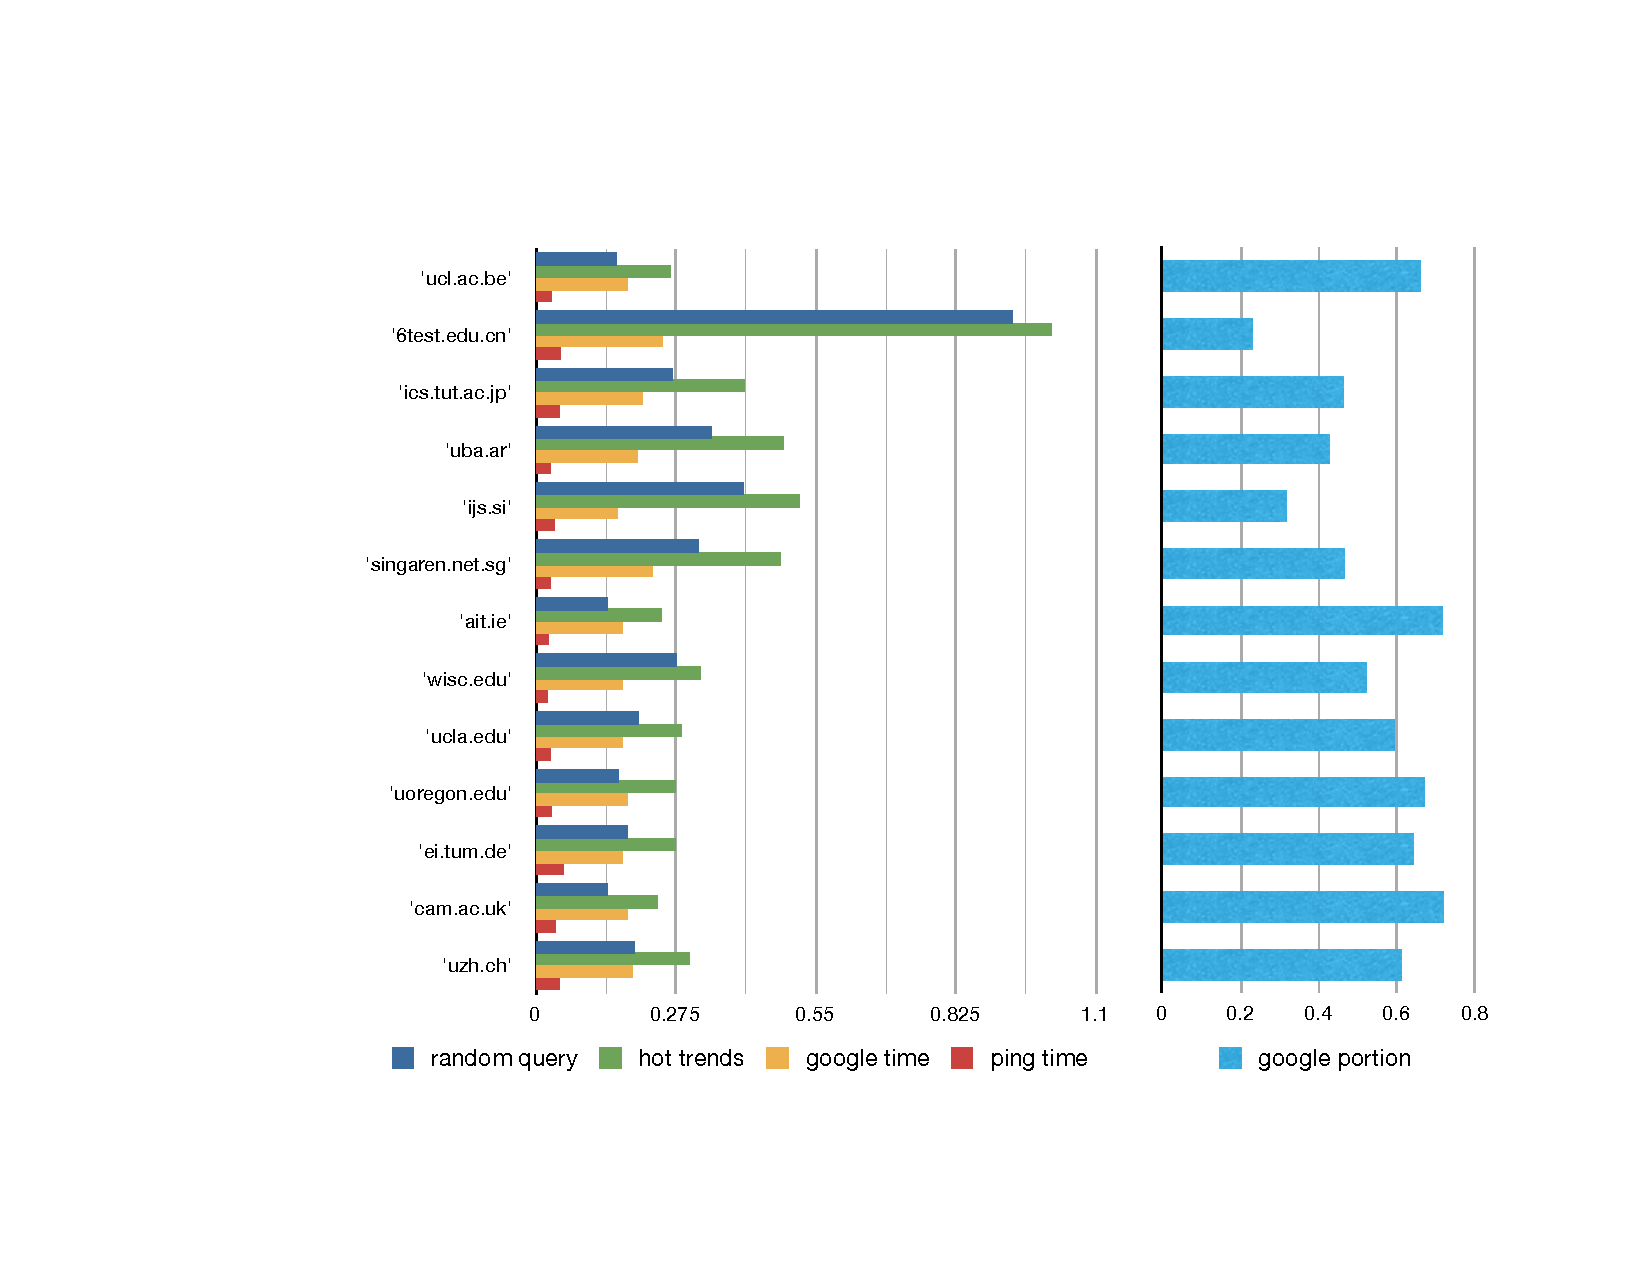
\includegraphics[width=\linewidth]{../figs/data_center.pdf}
  \caption{The latency measured in DC conversation experiments}
  \label{fig:data_center}
\end{figure}

%%% Local Variables: 
%%% mode: latex
%%% TeX-master: "main"
%%% End: 


\section{Latency in Cellular Networks}

\subsection{Methodology and Experiment}
\label{sec:methodology}

There are several existing tools for measuring mobile network performance \cite{speedtest, huang2011mobiperf}; however, these techniques are often too narrow in scope and can only be applied in a limited manner. We shy away from developing a whole new suite of measurement tools for mobile contexts given the fact that there are many general tools for understanding network performance (\ref{sec:tools}). We aim to reuse these existing tools in our study. We utilize mobile devices (in this case a smart phone) as a tethered network interface to a measurement system. The mobile device will serve as the first hop, allowing use to use existing tools and techniques to perform measurements. We utilize USB tethering to minimize the possibility of interference. As we will show in our data analysis, the latency of the first hop is negligible. Fig.\,\ref{fig:mobile_networks_method} illustrates our technique for probing cellular networks.

\begin{figure}
  \centering
  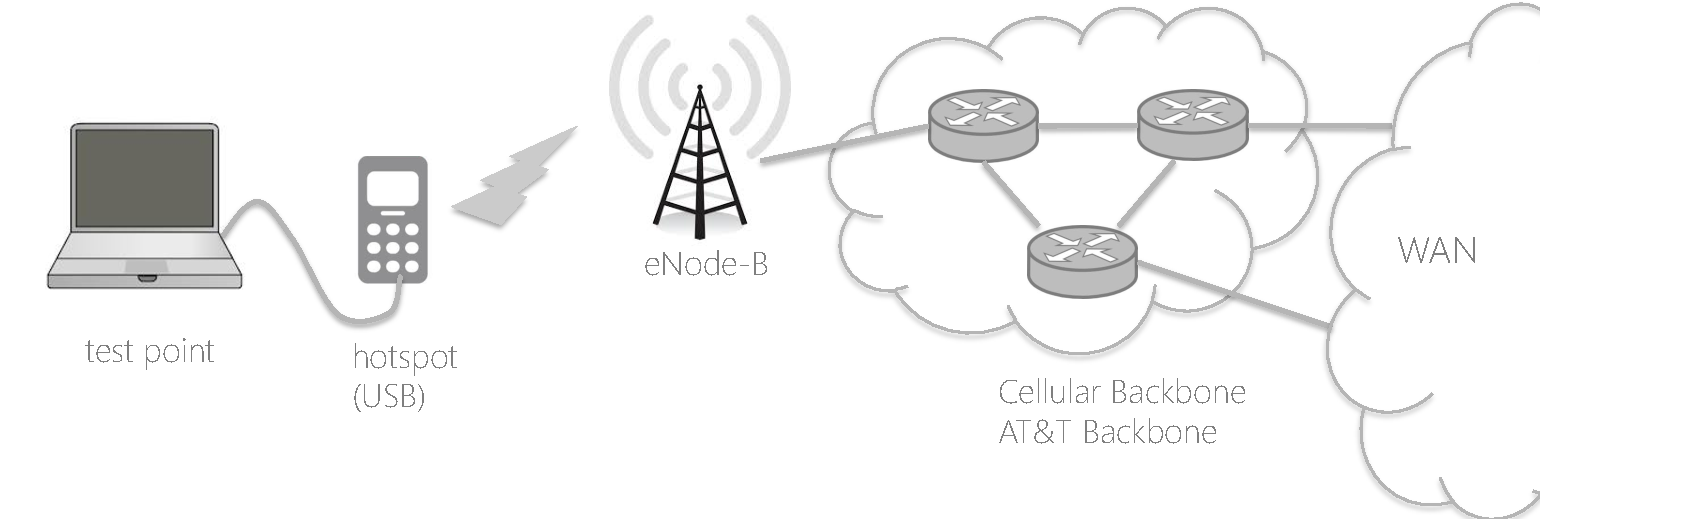
\includegraphics[width=\linewidth]{../figs/mobile_networks_method.pdf}
  \vspace{-1em}
  \caption{Mobile device USB tethered computer to perform {\textit traceroute}. This allows us to calculate the per-hop latency in cellular backbone.}
  \label{fig:mobile_networks_method}
\end{figure}

We utilize {\textit traceroute} to quantify the latency for each hop within cellular networks. The targets for {\textit traceroute} are the top 1000 websites. Since we are only interested in the cellular backbone networks, we limit the maximum hop count of {\textit traceroute} to 13. We also perform Autonomous System Number (ASN) lookups for each hop encountered. Fig.\,\ref{fig:traceroute} shows an example trace to Google.

\begin{figure}[!htb]
  \centering
  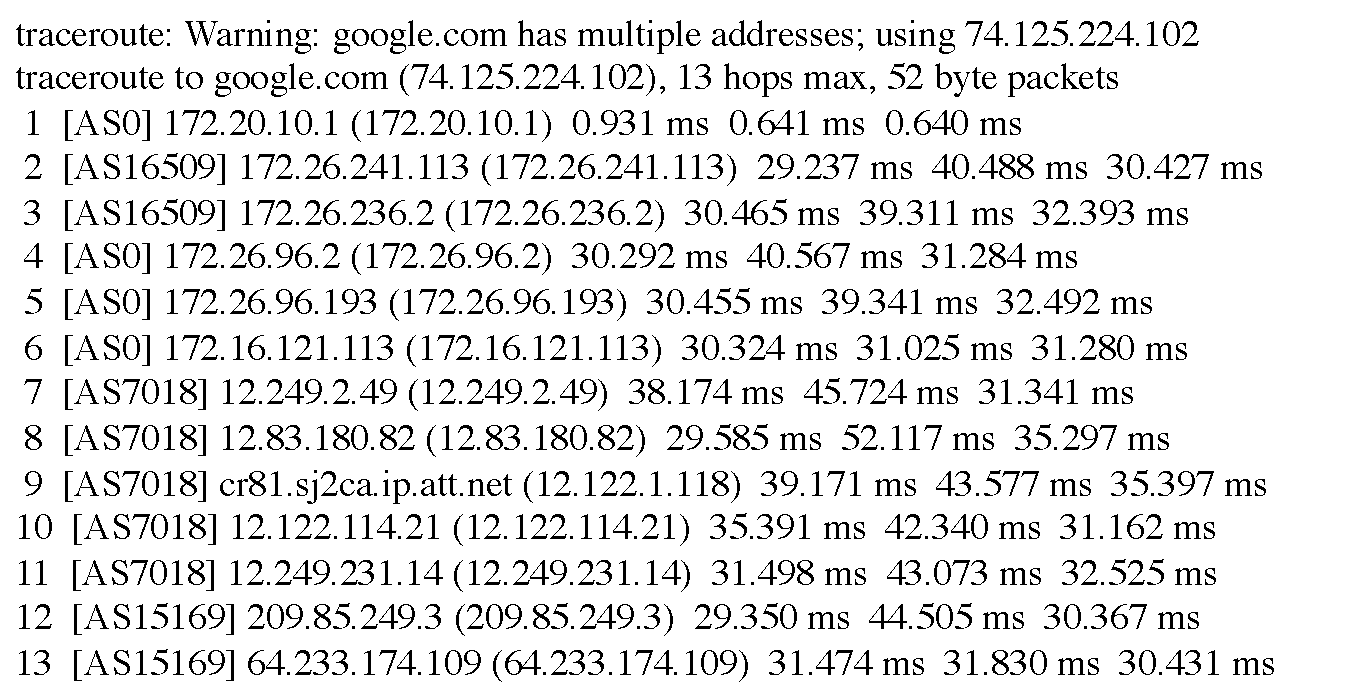
\includegraphics[width=1.1\linewidth]{../figs/traceroute.pdf}
  \vspace{-1em}
  \caption{Example {\textit traceroute} log from an AT\&T iPhone in Berkeley, maximum hop limited to 13, with ASN look-up turned on.}
  \label{fig:traceroute}
\end{figure}


The measurement was conducted between Apr.\,11 and Apr.\,24 (during periods in which we had access to a modem device). In total we have collected 191886 measurements, with each including a timestamp, received signal strength indication (RSSI), radio type (LTE or 4G-LTE), the traceroute hop number, ASN, hostname, host IP, and the specific delay. It is worth mentioning that the timestamp, RSSI and radio type are the same for each measurement. The reason is due to the difficulty in accessing RSSI and radio type programmatically. The we must manually record this data when performing the measurements.

Over the course of the experiment, we performed measurements while driving to and from San Francisco (SF). We expand on these results in the analysis section. 

\subsection{Analysis}
\label{sec:analysis}

We being with an example trace to Google (Fig.\,\ref{fig:traceroute}). As you can see, the first hop has an IP address $172.20.10.1$, and latencies 0.931 ms, 0.641 ms, 0.640 ms; this is the iPhone used for USB hotspot. Throughout the experiment, the latency introduced by this USB link is generally small, within 1 ms. Then the second hop reaches out to the first layer 3 router within AT\&T's cellular network. In the LTE architecture, the Evolved Node B (eNode-B) (Fig.\,\ref{fig:mobile_networks_method}) communicates directly with User Equipment (UEs), but it does not have layer 3 semantics. It is the access gateway (AGW) \footnote{AGW also provides termination of the LTE bearer, acts as a mobility anchor point for the user plane. Other key logical functions including MME (Mobility Management Entity) for the Control Plane and SAE PDN GW (System Architecture Evolution Packet Data Network GateWay) for the User Plane \cite{nortel}} that works on IP layer. Afterwards, the packet will enter AT\&T's cellular backbone, traversing routers either with private IP -- 172.16/12 \cite{rekhterrfc}, or with AT\&T's prefix -- 12/8. Interestingly, the ASN reported by {\textit traceroute} on the second and third hop is from Amazon's AS (AS16509). This might be due to some incorrect information in the ASN look-up. At hop 12, the route exits AT\&T's network and enters Google's AS.

This same pattern holds for many other traces. We aggregate them to answer the following question: what are the properties of AT\&T's cellular backbone? Is the latency stable, and are the routes stable? We plot the graph in Fig\,\ref{fig:mobile_latency}. The top figure shows the latency experienced on each hop (the horizontal axis is hop number, and vertical axis is latency in milliseconds). The red bar is the mean value for each hop, and the blue error bar is 5th and 95th percentile. We have also noted the mean value on top of each bar. The bottom figure displays the routing stability within the cellular networks. We mark each different router IP in a unique color for each hop. the portion of that color within each bar represents the portion of {\textit traceroute} responses received from that router for that hop. Again, it is important to note that the first hop is the iPhone through USB tethering.

\begin{figure}
  \centering
  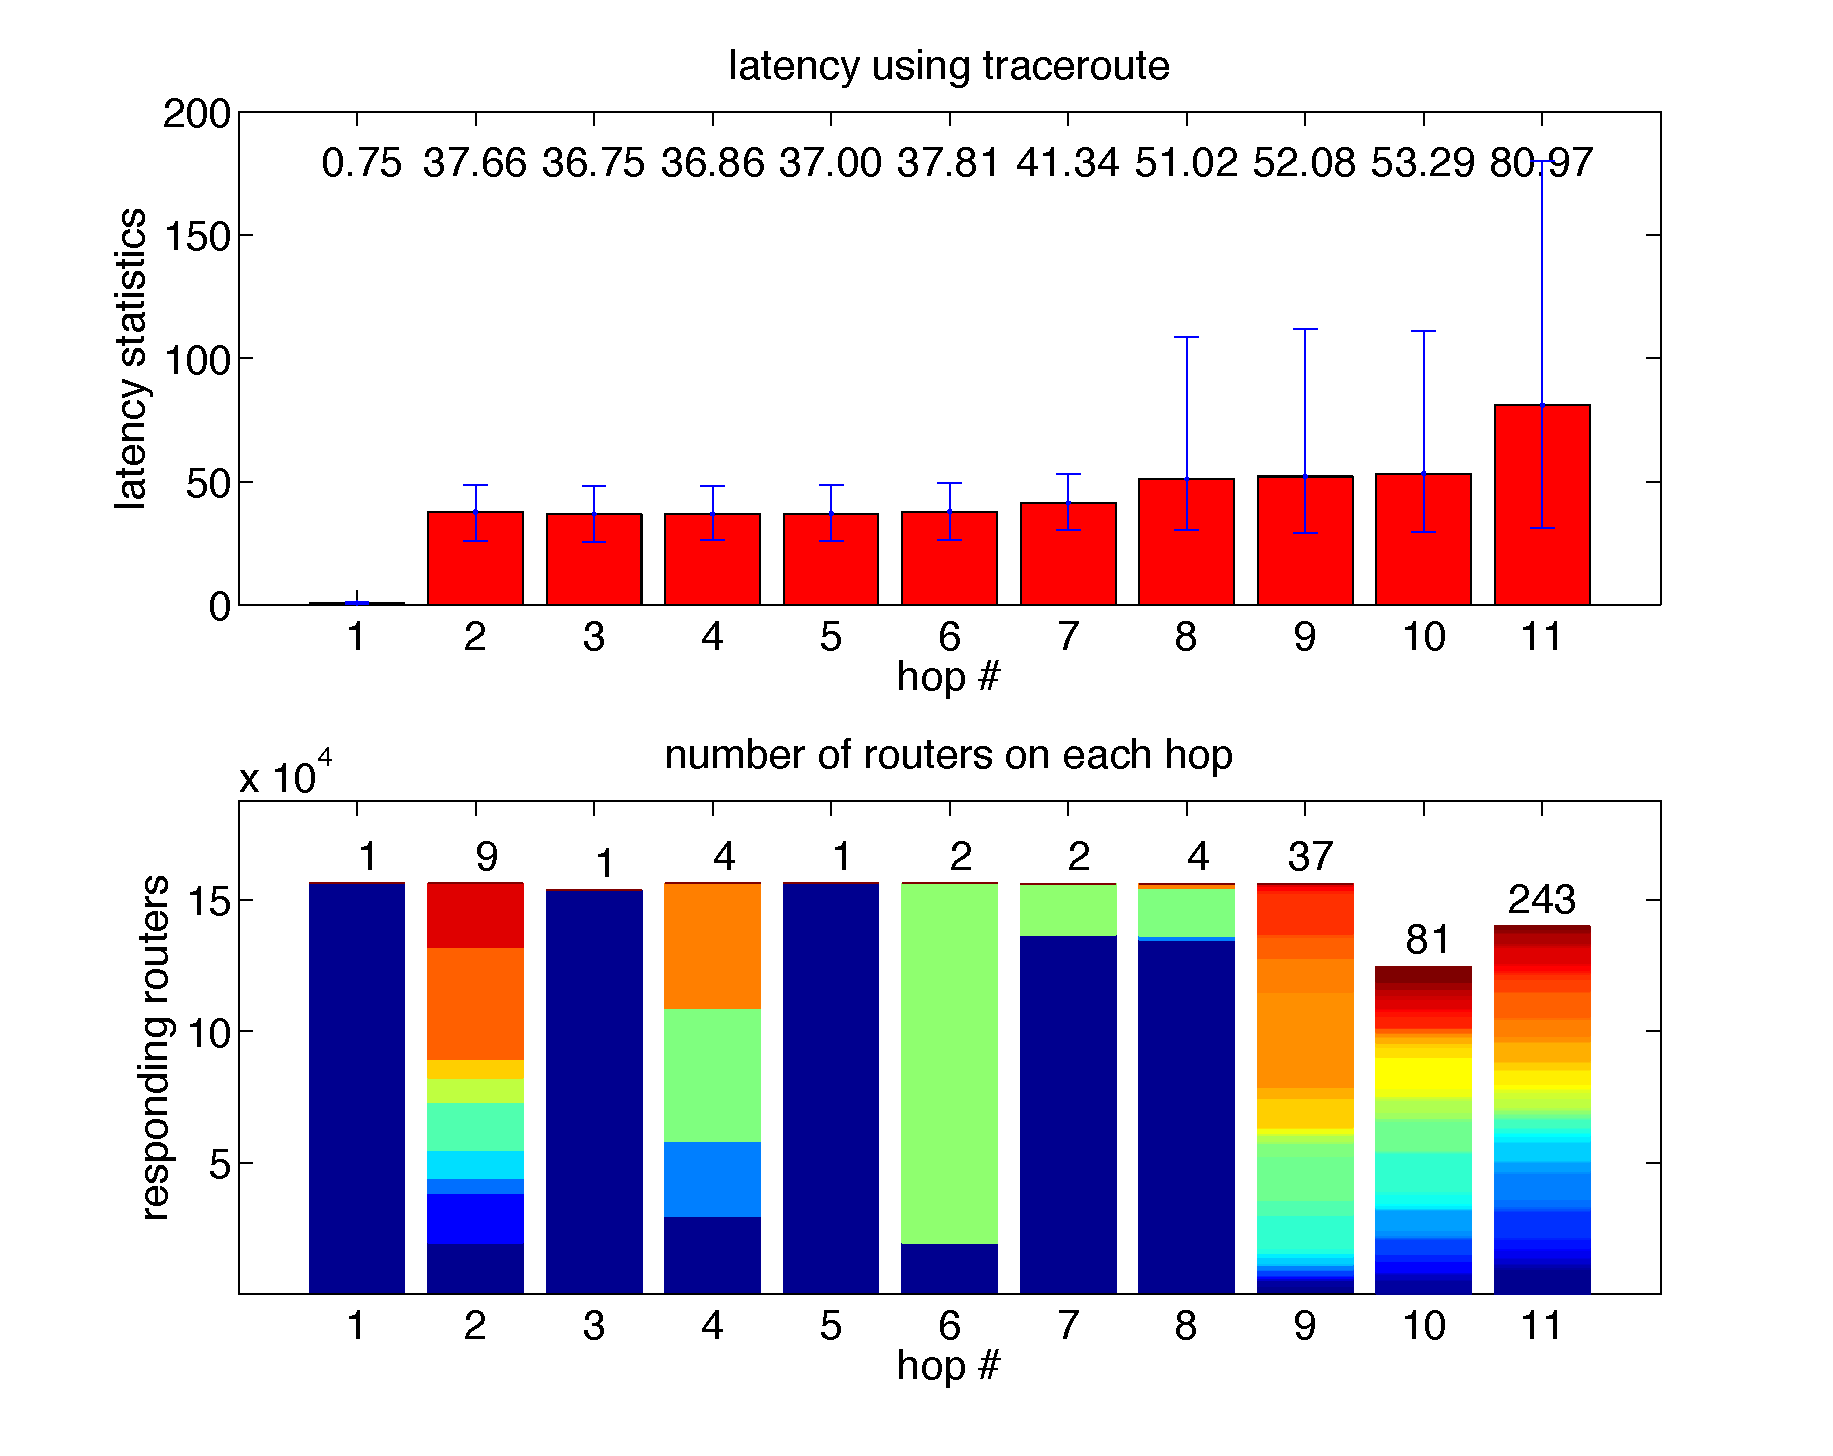
\includegraphics[width=\linewidth]{../figs/mobile_latency.pdf}
  \vspace{-1em}
  \caption{(Top) Latency measured in each hop of AT\&T cellular networks; (Bottom) The number of routers that responded on each hop}
  \label{fig:mobile_latency}
\end{figure}

We have found that within the cellular backbone and AT\&T's network (from the 2nd hop to 7th hops), the latencies are fairly stable at around 40 ms with variation of about 15 ms. There are also relatively few routers on a given hop. The second hop has 9 different responders, which are likely AGWs behind the eNode-B. They do not seem to change based on your location (as you can see in Fig\,\ref{fig:mobile_mobile} when we were moving between Berkeley and SF). We conjecture that the fourth hop might be comprised of four load balancers, as the fifth hop is consistent across all the measurements. After first 7 hops, the latency experiences a large increase, and the number of routers on each hop also increase dramatically.

\begin{figure}
  \centering
  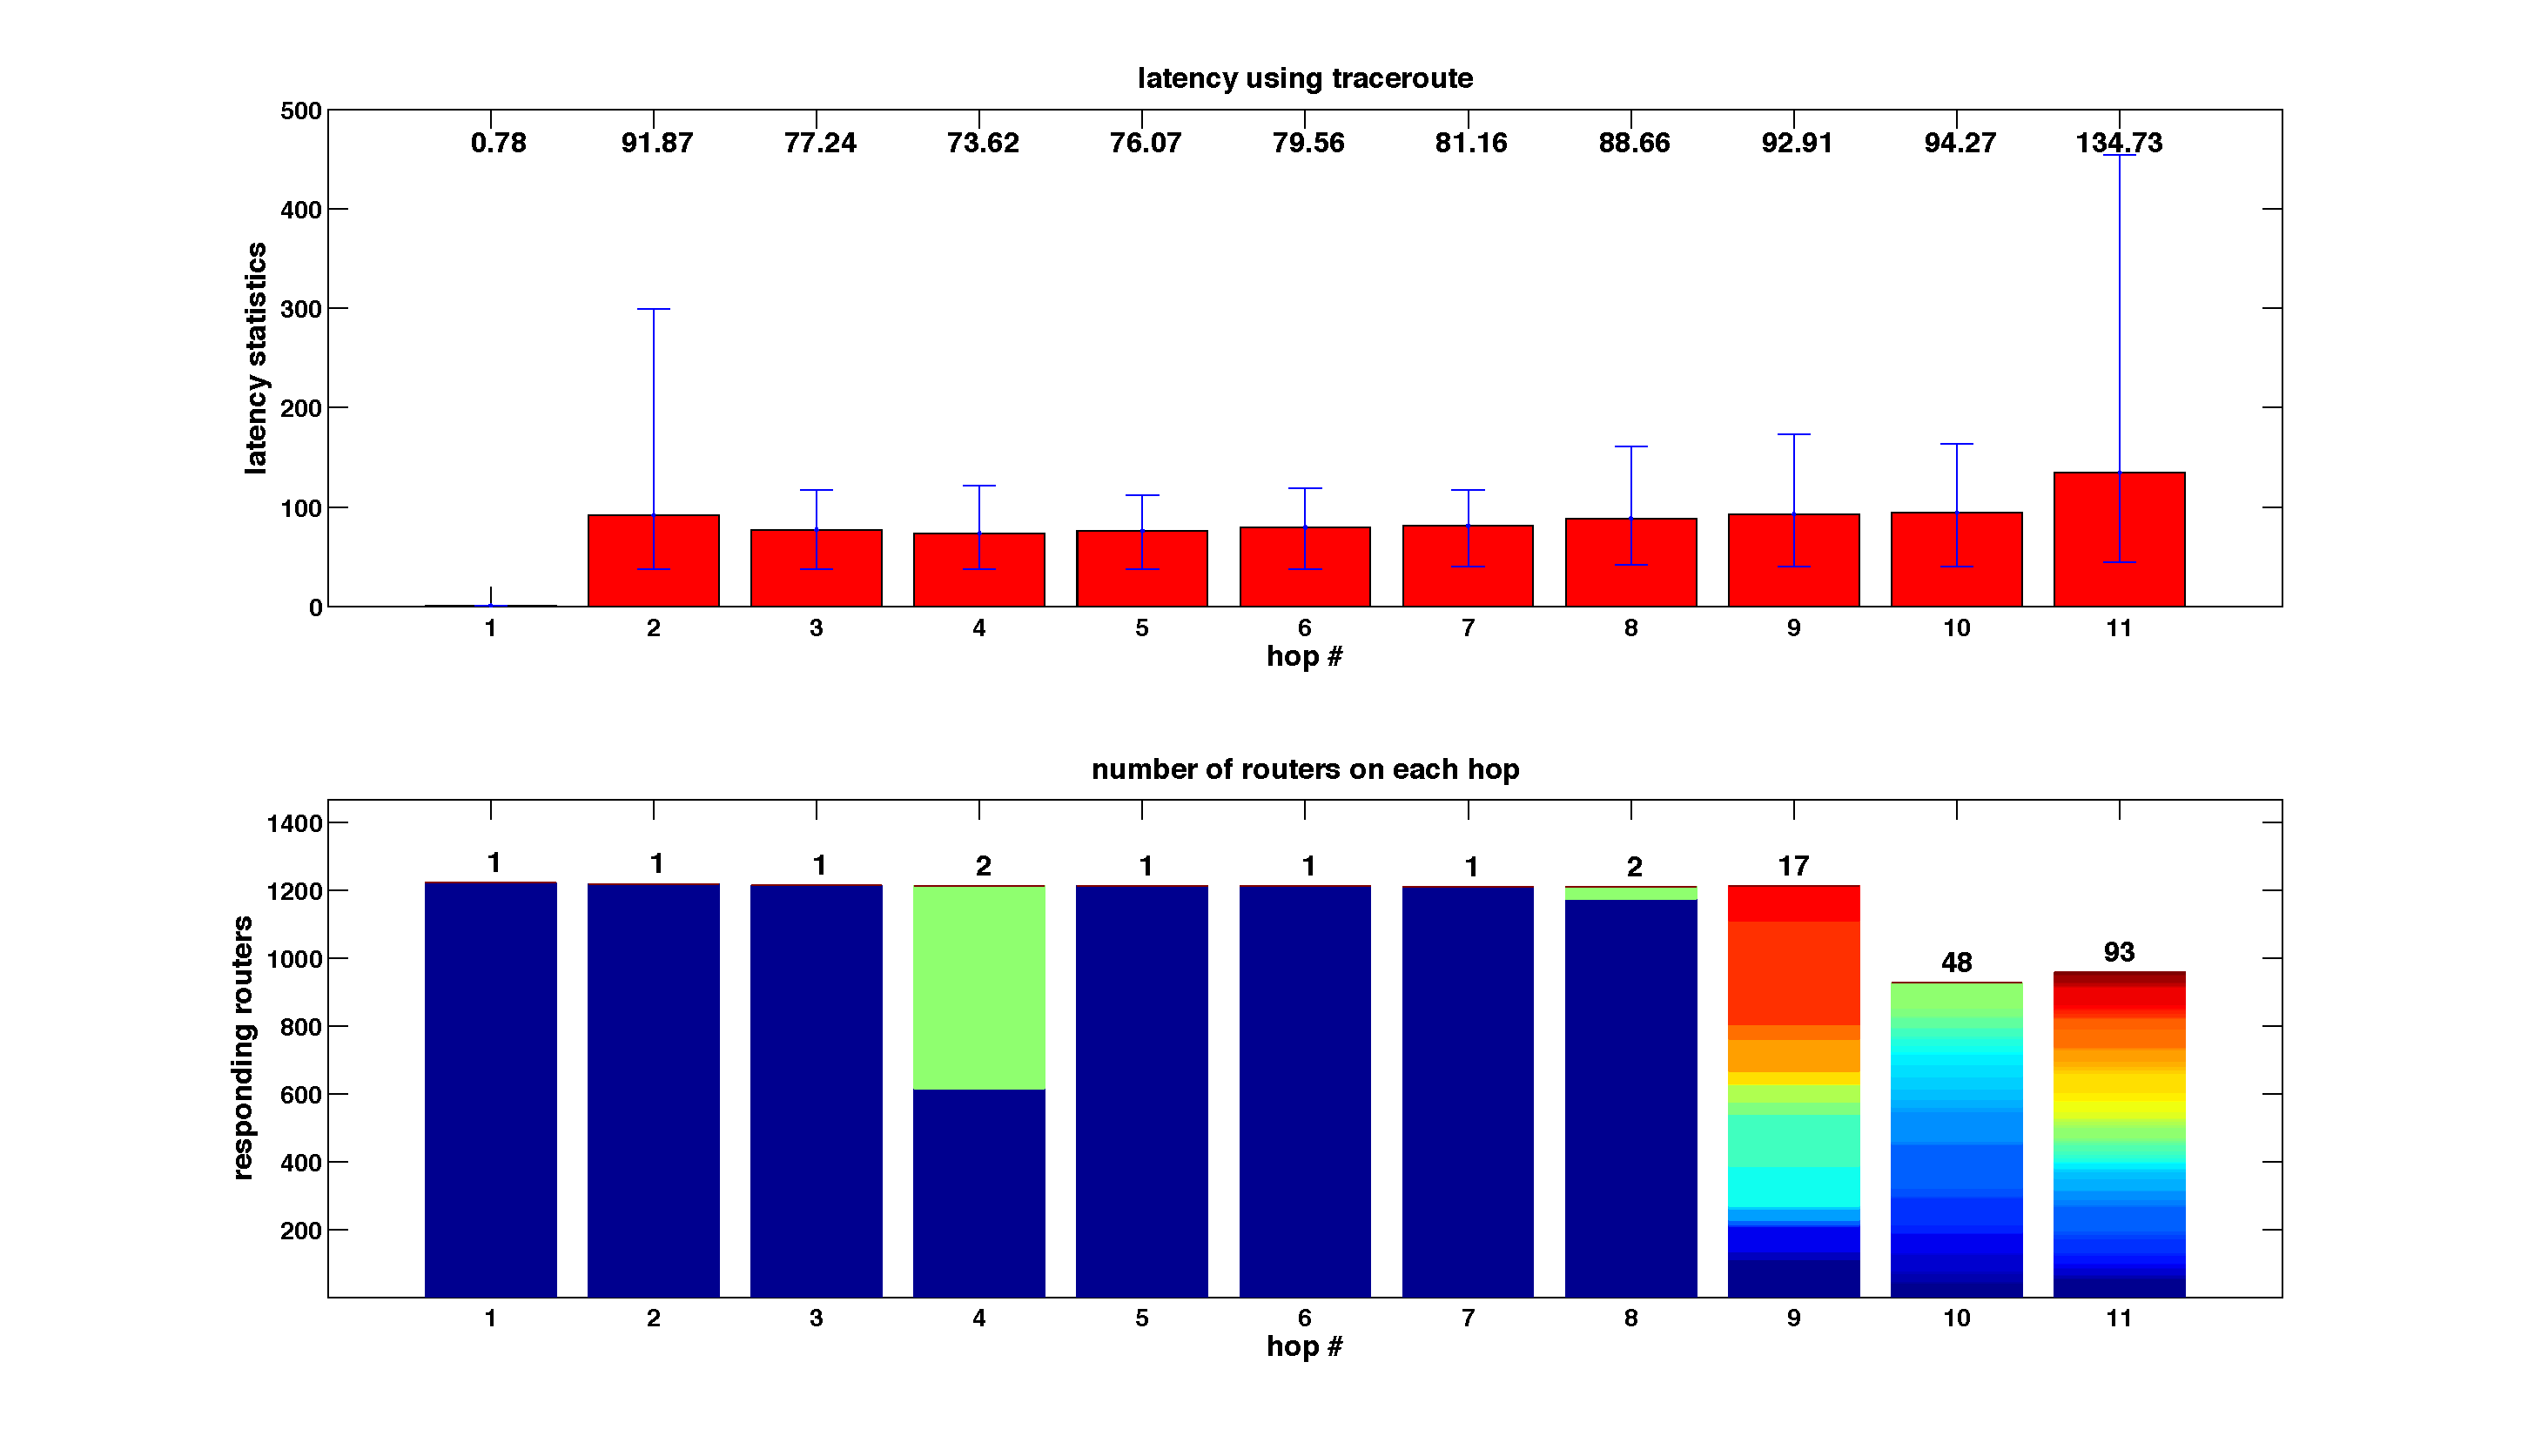
\includegraphics[width=\linewidth]{../figs/mobile_sfo.pdf}
  \vspace{-1em}
  \caption{Measurements conducted while moving between Berkeley and San Francisco.\\ (Top) latency measured in each hop of AT\&T cellular networks; (Bottom) the number of responding routers on each hop}
  \label{fig:mobile_mobile}
\end{figure}

From Fig.\,\ref{fig:mobile_mobile}, we find that the latencies are significantly larger when compared to Fig.\,\ref{fig:mobile_latency}. We believe that this is in part due to a difference in radio access technology -- during the majority of the journey, the mobile device utilized the 4G (HSDPA+) network rather than LTE. As can be seen, the latency on the second hop has increased significantly; we believe mobility accounts for part of the degradation. Once again the routing within the cellular backbone is fairly stable.

To further understand routing stability, we evaluate each trace. In a single {\textit traceroute} log, the routing might change; this rapidly-variable routing is called fluttering \cite{paxson1997measurements}. For each hop, we determine how many different routes the packet has taken, and draw this in a stacked bar plot (Fig.\,\ref{fig:mobile_fluttering}). The horizontal axis the hop number and the vertical axis counts the number of different routes in our measured data. For most of the routes within AT\&T's cellular backbone, the routes are fairly stable. When approaching the WAN (starting from hop 11), routing fluttering happens more frequently (likely due to the crossing of AS boundaries).

\begin{figure}
  \centering
  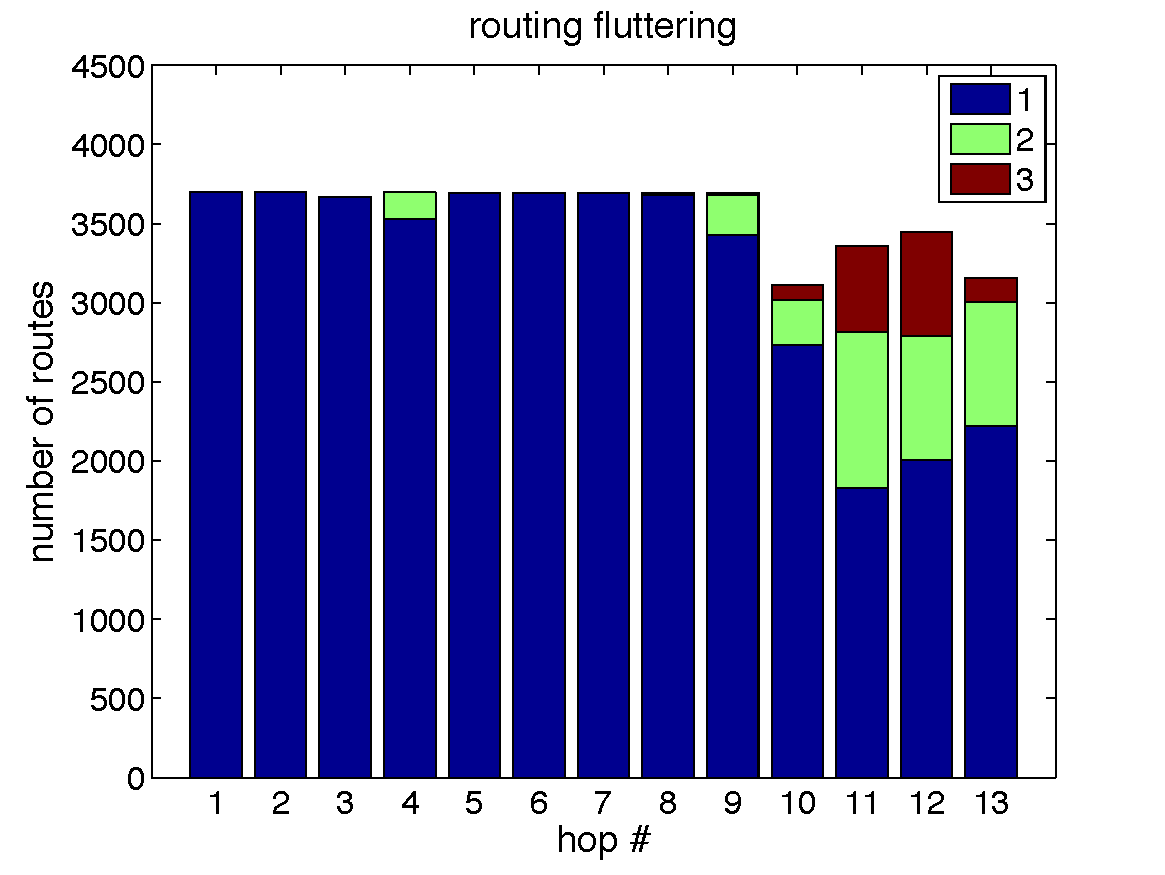
\includegraphics[width=\linewidth]{../figs/mobile_fluttering.pdf}
  \vspace{-1em}
  \caption{Routing fluttering within AT\&T cellular networks}
  \label{fig:mobile_fluttering}
\end{figure}

%%% Local Variables: 
%%% mode: latex
%%% TeX-master: "main"
%%% End: 


\section{Discussion}
\label{sec:discussion}


%%% Local Variables: 
%%% mode: latex
%%% TeX-master: "main"
%%% End: 


\section{Conclusion}
\label{sec:conclusion}


%%% Local Variables: 
%%% mode: latex
%%% TeX-master: "main"
%%% End: 


% \section{Acknowledgments}

\bibliographystyle{abbrv}
\bibliography{Measurement}

\end{document}